%\documentclass[onecolumn]{emulateapj}
\documentclass{emulateapj}
\newcommand{\beq}{\begin{equation}}
\newcommand{\eeq}{\end{equation}}
\newcommand{\hyd}    {{\rm H}}
\newcommand{\vobs}{v_{\rm obs}}
\newcommand{\hi}{H{\sc i}~}
\newcommand{\hii}{H{\sc ii}~}
\newcommand{\hia}{H{\sc i}}
\newcommand{\hiia}{H{\sc ii}}

\usepackage[colorlinks,urlcolor=blue,citecolor=blue,linkcolor=blue]{hyperref}
\usepackage{gensymb}
\usepackage{amsmath}
\usepackage{color}
%\usepackage{appendix}
\usepackage[titletoc,title]{appendix}
\usepackage{cleveref}


\makeatletter
\setlength{\@fptop}{0pt}
\setlength{\@fpbot}{0pt}
\setlength{\@fpsep}{0pt}
\makeatother

\newcommand{\citei}[1]{\citeauthor{#1} \citeyear{#1}}
\newcommand{\unit}[1]{\textrm{ #1}}
\newcommand{\kms}{km ${\rm s^{-1}}$}
\newcommand{\kmsa}{km ${\rm s^{-1}}$}
\newcommand{\citeia}[2]{\citeauthor{#1}~(\citeyear{#1};~#2)}

\newcommand\reye{\mathrm{Re}}
\newcommand\reym{\mathrm{Rm}}

\newcommand{\uphi}{\ensuremath{u_\phi}}
\newcommand{\rhat}{\ensuremath{\mathbf{\hat{r}}}}
\newcommand{\phihat}{\ensuremath{\mathbf{\hat{\phi}}}}
\newcommand{\zhat}{\ensuremath{\mathbf{\hat{z}}}}
\newcommand{\xhat}{\ensuremath{\mathbf{\hat{x}}}}
\newcommand{\yhat}{\ensuremath{\mathbf{\hat{y}}}}

\renewcommand{\topfraction}{0.85}
\renewcommand{\textfraction}{0.1}
\renewcommand{\floatpagefraction}{0.75}

\begin{document}

%\title{Weakly Nonlinear Analysis of the Standard and Helical Magnetorotational Instabilities in a Taylor Couette Flow}
\title{The Weakly Nonlinear Magnetorotational Instability} % maybe this is punchier?
\author{Clark, S.E.\altaffilmark{1}}
\author{Oishi, J.S. \altaffilmark{2,}\altaffilmark{3}}
%\author{Mac Low, M.-M.\altaffilmark{1,}\altaffilmark{2}}
\altaffiltext{1}{Department of Astronomy, Columbia University, New York, NY} 
\altaffiltext{2}{Department of Astrophysics, American Museum of Natural History, New York, NY}
\altaffiltext{3}{Department of Physics, SUNY Farmingdale}


\begin{abstract}
We conduct a formal weakly nonlinear analysis of the magnetorotational instability (MRI) in a Taylor Couette flow. This is a multiscale perturbative treatment of the nonideal, axisymmetric MRI near threshold, subject to realistic radial boundary conditions. We analyze both the standard MRI, initialized by a constant vertical background magnetic field, and the helical MRI, in which the base magnetic field contains an azimuthal component. We find that the evolution of the weakly nonlinear perturbation amplitude of the standard MRI is described by a real Ginzburg-Landau equation (GLE), while the amplitude of the helical MRI takes the form of a complex GLE.   
\end{abstract}

\section{Introduction}

The magnetorotational instability (MRI) drives angular momentum transport and turbulence in astrophysical disks. Its discovery by \citeauthor{Balbus:1991vs} (\citeyear{Balbus:1991vs}; actually a rediscovery of \citei{Chandrasekhar:1960wh}) was a breakthrough in the longstanding question of how efficient accretion can exist in the universe: that is, how matter collapsing onto a central body is able to coalesce despite the conservation of specific angular momentum. %The ubiquity of disks ...
The ubiquity of astrophysical disks suggests that systems both experience and overcome this centrifugal barrier, and accretion proceeds even in hydrodynamically stable disks, where molecular viscosity is vastly insufficient to drive angular momentum transport (\citei{Shakura:1973wg}). The MRI is excited by weak magnetic fields in differentially rotating fluids, and since its discovery it has been widely invoked to explain accretion in protoplanetary disks (see \citei{Armitage:2010} and references therein), binary systems (), and disks around black holes (), as well as jet and wind launching (\citei{Lesur:2013}), dynamos, etc (cite these)

%Magnetic fields were once assumed to have a stabilizing effect 

%The MRI is fundamental to our understanding of star formation, but its 
%- people make a number of simplifications, incl thin gap, shearing box, etc

%Despite the challenges inherent in studying the MRI, much progress has been made nu

Although the MRI is broadly important to many astrophysical systems, many of its general properties, and in particular its nonlinear saturation mechanism, remain poorly understood. The diversity of astrophysical systems which may permit the MRI admits an enormous parameter space to be explored. In protoplanetary disks, for example, the behavior and evolution of the MRI may change drastically depending on the properties of the magnetic field, the disk composition, disk geometry, and so forth. Numerical simulation of realistic disk physics is currently an area of intense focus, and is enabling the study of nonideal MHD effects, disk stratification, nonequilibrium chemistry, and other complex physics that does not lend itself easily to analytic study (\citei{Fleming:2003fs}, \citei{Bai:2011cm}, \citei{Flock:2013}, \citei{Suzuki:2014vh}, to name only a few). Still, computational costs inevitably constrain numerical approaches. MRI saturation is a complicated nonlinear problem which may depend on the assumptions and approximations adopted by simulations in nonobvious ways. Analytic methods can play a powerful role in elucidating the mechanisms responsible for MRI saturation. For instance, analytical approaches have revealed the mechanism that likely governs saturation in the ``shearing box" approximation. The shearing box is an oft-invoked local approximation in which a section of a disk is represented by solving the MHD equations in an isolated region subject to shear periodic boundary conditions. The shearing box is an inexpensive computational framework, and has been widely used to study many aspects of the MRI (). However, while the MRI is a local instability, certain properties of the local problem are not generic to the global problem. In the shearing box, linear evolution is dominated by a class of MRI mode known as channel modes. These are linear modes which also happen to be exact solutions to the \textit{nonlinear} local MRI equations. Runaway growth is avoided in this paradigm by the instability of the channel modes themselves, which are destroyed by parasitic (secondary) instabilities (\citei{Goodman:1994ul}, \citei{Pessah:2010ic}). The growth of parasitic modes provides a saturation avenue for channel mode-dominated flows, yet this is unlikely to be the dominant saturation mechanism in laboratory experiments or astrophysical disks, as channel modes are artificially over-prominent in the shearing box (e.g. \citei{Latter:2015}). Thus while the shearing box may accurately approximate many features of the global MRI, the saturation mechanism is not among them. 

%Because of the MRI's complexity, analytical treatments of the MRI use some combination of convenient approximations, such as ideal MHD, linearized equations, expedient boundary conditions, and simplified geometries. In particular, much of the analytical work on MRI saturation has focused on local approximations, often representing a section of a disk by solving the MHD equations in an isolated region subject to shear periodic boundary conditions (the ``shearing box"). The shearing box is an inexpensive computational framework, so is used by many numerical MRI studies as well. However, while the MRI is a local instability, certain properties of the local problem are not generic to the global problem. In the shearing box, linear evolution is dominated by a class of MRI mode known as channel modes.  %Channel modes, a class of MRI mode that dominates MRI evolution and saturation in the local approximation, are artificially over-prominent in the shearing box (e.g. \citei{Latter:2015}). 
%These are linear modes which also happen to be exact solutions to the \textit{nonlinear} local MRI equations. Runaway growth is avoided in this paradigm by the instability of the channel modes themselves, which are destroyed by parasitic (secondary) instabilities (\citei{Goodman:1994ul}, \citei{Pessah:2010ic}). The growth of parasitic modes provides a saturation avenue for channel mode-dominated flows, yet this is unlikely to be the dominant saturation mechanism in laboratory experiments or astrophysical disks, as channel modes are artificially over-prominent in the shearing box (e.g. \citei{Latter:2015}). 

The theory we develop here employs realistic radial boundary conditions, and so MRI modes are global and channel modes are not present. A number of saturation mechanisms have been proposed for the MRI which do not rely on channel modes dominating the flow. The MRI feeds off of the free energy from differential rotation, and so a modification of the background shear may cause saturation (e.g. \citei{Knobloch:2005ba}, \citei{Umurhan:2007hs}). The MRI may transfer its free energy into the magnetic field, and saturate when the field is too strong to be susceptible to the MRI (e.g. \citei{Ebrahimi:2009ey}). The MRI may saturate differently depending on the particular parameter regime under investigation, and so our challenge is not only in identifying possible saturation mechanisms, but in understanding how and when each applies in different astrophysical environments.

Our investigation is astrophysically motivated, but we also intend our theory to be relevant to laboratory experiments. Several experimental efforts are attempting to observe the MRI in the laboratory, which would allow the study of a crucial astrophysical phenomenon in a controlled setting. Unfortunately, detection of the MRI has so far proven elusive. \citei{Sisan:2004ig} claimed to detect the MRI in a spherical Couette flow, but most likely detected unrelated MHD instabilities instead (\citei{Hollerbach:2009ig}, \citei{Gissinger:2011td}). Most relevant to our work is the Princeton Plasma Physics Laboratory (PPPL) MRI Experiment, a liquid gallium Taylor-Couette flow exposed to an axial magnetic field (\citei{Ji:2001kd}). Some theoretical work designed to complement the Princeton MRI experiment involves direct simulation of the experimental conditions, much of it focused on the specific challenges in identifying MRI signatures despite apparatus-driven spurious flows (e.g. \citei{Gissinger:2012gc}). In particular, the vertical endcaps on a laboratory MRI apparatus drives meridional flows which both inhibit the excitement of MRI and obscure its detection. The Princeton MRI experiment employs split, independently rotating endcaps to mitigate these flows (\citei{Schartman:2009df}). Our work here assumes an infinite vertical domain, an idealization that is theoretically expedient but experimentally impractical. However, our setup is designed to be an accurate treatment of the radial dimension of the flow in a Taylor Couette apparatus like the one used in the Princeton MRI experiment. 

Many investigations of the MRI use the ``narrow gap" approximation, in which the radial extent of the fluid channel is taken to be much smaller than the radius of curvature. That is, for a channel center $r_0$ bounded by inner and outer radii $r_1$ and $r_2$, respectively, the narrow gap approximation applies when $r_0 \gg (r_2 - r_1)$. The narrow gap approximation simplifies the MRI equations by excluding curvature terms, because the flow through a narrow gap can be taken to be approximately linear in $\phi$, i.e. Cartesian. Previous investigations into the weakly nonlinear MRI have used this narrow gap approximation (\citei{Umurhan:2007dz}, \citei{Umurhan:2007hs}, \citei{Clark:2016}). In this work we undertake the first (to our knowledge) weakly nonlinear analysis of the MRI in the wide gap regime, where the channel width may be comparable to or larger than its distance from the center of rotation.

Because we include curvature terms, our theory is also relevant to the helical magnetorotational instability (HMRI). Discovered by \citeauthor{Hollerbach:2005tr} (\citeyear{Hollerbach:2005tr}), the HMRI is an overstability in which the background magnetic field is helical. The HMRI currently occupies a special place in the MRI puzzle. The HMRI has been proposed as a method of awakening angular momentum transport in the ``dead zones" of protoplanetary disks where the magnetic Prandtl number ($Pm = \nu/\eta$) becomes very small. However the rotation profiles needed to excite HMRI may be prohibitively steeper than Keplerian depending on the boundary conditions, and so its role in astrophysical disks is currently debated (\citei{Liu:2006}, \citei{Rudiger:2007}, \citei{Kirillov:2013}). The HMRI is significantly easier to excite in a laboratory setting than the standard MRI, and has already been detected in the laboratory by the Potsdam Rossendorf Magnetic Instability Experiment (PROMISE; \citei{Stefani:2006iv}, \citei{Stefani:2009hp}). %The standard MRI has yet to be detected in the laboratory, although several plasma experiments are making progress.

In this work we explore the behavior of the viscous, dissipative MRI in a cylindrical geometry close to threshold, making explicit comparisons to the standard MRI behavior in the thin-gap regime. 

\begin{figure}
\centering
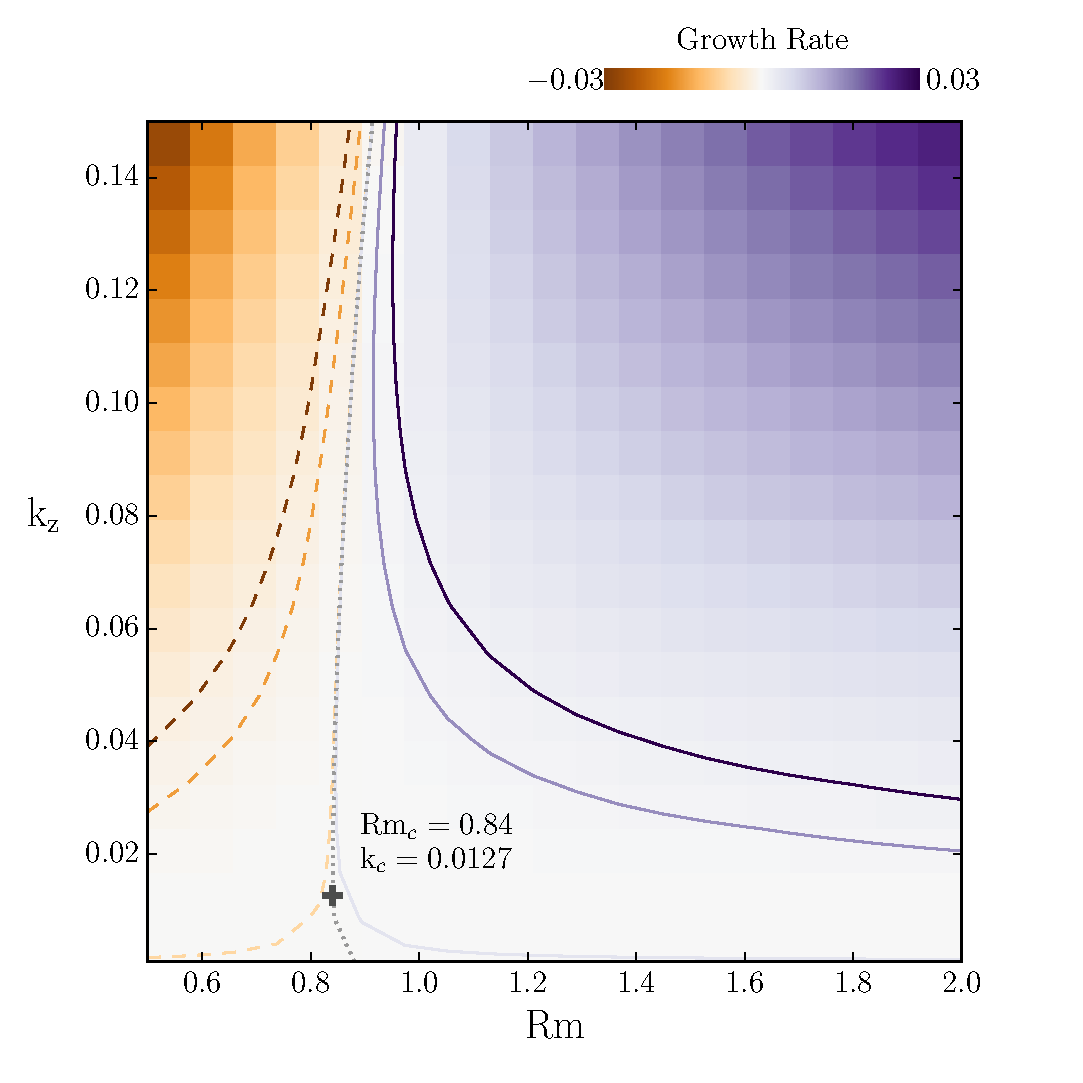
\includegraphics[width=\columnwidth]{../figures/widegap_paramspace_crit_params_Pm_1E-3}
\caption{Growth rates in the ($\reym, k_z$) plane. Color map shows growth rate found by solving the linear eigenvalue problem for each ($\reym, k_z$) in the grid. The eigenvalue problem was solved for the widegap parameters listed in Table \ref{table:parameters}. Overlaid contours show growth rates at [-2E-3, -1E-3, -1E-5, 1E-5, 1E-3, 2E-3], where dashed contours represent negative values. The gray dotted line shows the interpolated marginal stability curve. The critical parameters $\reym_c = 0.84$ and $k_c = 0.0127$ correspond to the smallest parameter values that yield a zero growth rate.}\label{fig:growth_rates}
\end{figure}

\section{Wide Gap Equations}

The basic equations solved are the momentum and induction equations,

\beq\label{momentum}
%\begin{split}
\partial_t \mathbf{u} + \mathbf{u} \cdot \nabla \mathbf{u} = -\frac{1}{\rho}\nabla P - \nabla\Phi + \frac{1}{\rho} \left(\mathbf{J}\times\mathbf{B}\right) + \nu\nabla^2 \mathbf{u} 
%\end{split}
\eeq

and

\beq\label{induction}
\partial_t \mathbf{B} = \nabla \times \left(\mathbf{u} \times \mathbf{B}\right) + \eta\nabla^2\mathbf{B},
\eeq

where $P$ is the gas pressure, $\nu$ is the kinematic viscosity, $\eta$ is the microscopic diffusivity, $\nabla\Phi$ is the gravitational force per unit mass, and the current density is $\mathbf{J} = \nabla\times\mathbf{B}$. We solve these equations subject to the incompressible fluid and solenoidal magnetic field constraints,

\beq
\label{eq:incompressibility}
\nabla \cdot \mathbf{u} = 0
\eeq

and 

\beq
\label{eq:solenoid}
\nabla \cdot \mathbf{B} = 0.
\eeq

We perturb these equations axisymmetrically in a cylindrical $(r, \phi, z)$ geometry, i.e. $\mathbf{u} = \mathbf{u_0} + \mathbf{u_1}$ and $\mathbf{B} = \mathbf{B_0} + \mathbf{B_1}$, where $\mathbf{u_0}$ and $\mathbf{B_0}$ are defined below. We define a Stokes stream function $\Psi$ such that 

\beq
  \label{eq:stokes}
  \mathbf{u_1} \, = \, \left[\begin{matrix}
\frac{1}{r} \partial_z \Psi\ \rhat\\
\uphi \ \phihat\\
-\frac{1}{r} \partial_r \Psi\ \zhat\\
\end{matrix}\right],
\eeq

and define the magnetic vector potential $A$ analogously. These definitions automatically satisfy Equations \ref{eq:incompressibility} and \ref{eq:solenoid} for axisymmetric disturbances. We note that in the linearized equations, streamfunctions of the form $u_x = \partial_z \Psi$, $u_z = -(\partial_r + \frac{1}{r}) \Psi$, and the corresponding definitions of the magnetic vector potential, are convenient choices, but this does not hold true for the nonlinear terms because of the incommutability of $\partial_r$ and $\partial_r + \frac{1}{r}$. 

The astrophysical magnetorotational instability operates in accretion disks and in stellar interiors, environments where fluid rotation is strongly regulated by gravity. In accretion disks, differential rotation is imposed gravitationally by a central body, so the rotation profile is forced to be Keplerian. Clearly a gravitationally enforced Keplerian flow is inaccessible to laboratory study, so differential rotation is created by rotating an inner cylinder faster than an outer cylinder (a Taylor-Couette setup). For a nonideal fluid subject to no-slip boundary conditions, the base flow is

\begin{equation}
  \label{eq:couette_flow}
  \Omega(r) = c_1 + \frac{c_2}{r^2},
\end{equation}
where $c_1 = (\Omega_2 r^2_2 - \Omega_1 r^2_1)/(r^2_2 - r^2_1)$, $c_2 = r^2_1 r^2_2 (\Omega_1 - \Omega_2)/(r^2_2 - r^2_1)$, and $\Omega_1$ and $\Omega_2$ are the rotation rates at the inner and outer cylinder radii, respectively. In the laboratory, $r_1$ and $r_2$ are typically fixed by experimental design. However $\Omega_1$ and $\Omega_2$ may be chosen such that the flow in the center of the channel is approximately Keplerian. Defining a shear parameter $q$, we see that for Couette flow,
\begin{equation}
  \label{eq:couette_q}
  q(r) \equiv -\frac{d \ln \Omega}{d \ln r} = \frac{2 c_2}{c_1 r^2 + c_2}.
\end{equation}

\begin{figure*}
\centering
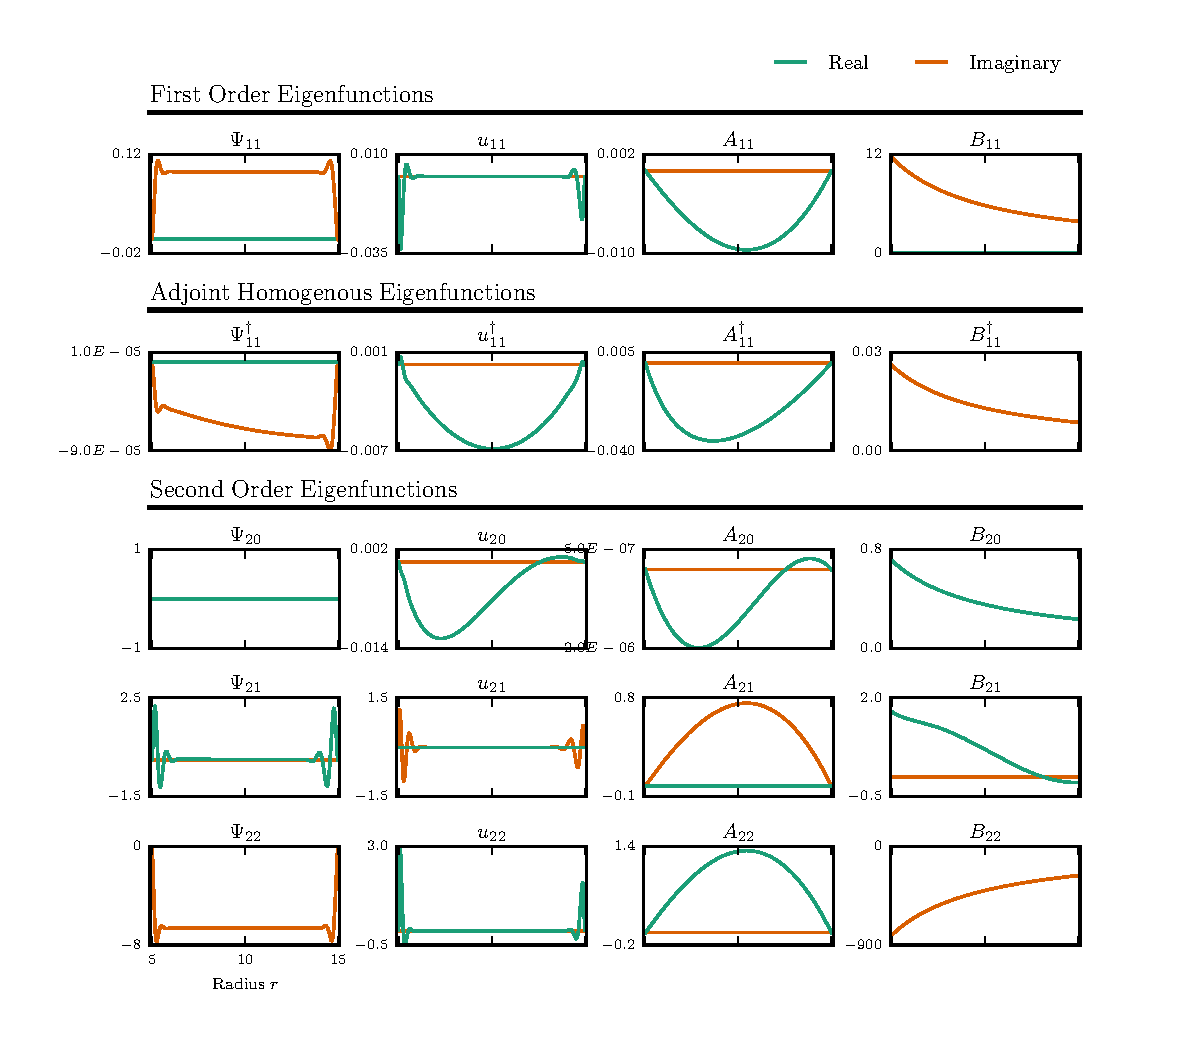
\includegraphics[width=\textwidth]{../python/widegap/figures/orders_1_2_widegap_fiducial_eigenfunctions.pdf}
\caption{Eigenfunctions of the first order equations, first order adjoint homogenous equations, and second order equations. We use our fiducial parameters for the standard MRI ($\xi = 0$). First-order eigenfunctions are normalized such that they are either purely real or purely imaginary, and such that $\int \Psi_{11} \mathrm{d}r = 1$. Adjoint homogenous eigenfunctions are normalized such that $\left< V_{11}^\dagger \cdot \mathcal{D} V_{11} \right> = 1$.}\label{fig:linear_eigenfunctions}
\end{figure*}

\begin{figure*}
\centering
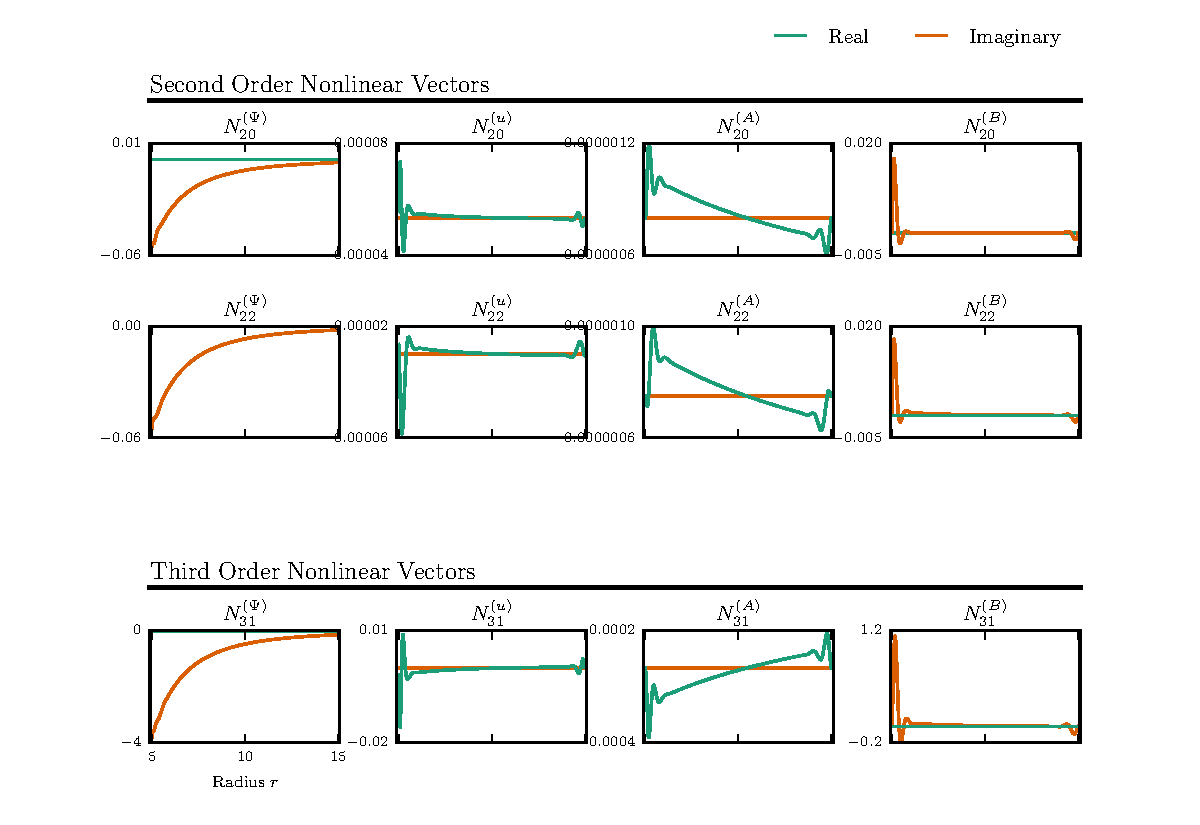
\includegraphics[width=\textwidth]{../python/widegap/figures/nonlinear_2_3_widegap_fiducial_eigenfunctions.pdf}
\caption{Nonlinear terms $N_2$ and $N_3$ for our fiducial standard MRI parameters.}\label{fig:N2_N3}
\end{figure*}

Thus through judicious choice of cylinder rotation rates, we can set $q(r_0) = 3/2$, for quasi-Keplerian flow. Note that the narrow gap approximation imposes a linear shear (constant $q$). Our base velocity is $\mathbf{u_0} = r\Omega(r) \phihat$. We initialize a magnetic field $\mathbf{B_0} = B_0 \zhat + B_0 \xi \frac{r_0}{r} \phihat$, so that the base magnetic field is axial when $\xi = 0$ and otherwise helical. 

In this work we will focus our findings on two fiducial parameter sets, one for the standard MRI (hereafter SMRI) where $\xi = 0$ and one for the helical MRI (hereafter HMRI). We choose the SMRI parameters to be comparable to the case explored in \citei{Umurhan:2007hs}, with the geometric parameters of \citei{Goodman:2002ix}. The HMRI parameters were chosen to be comparable to \citei{Hollerbach:2005tr}. Our fiducial parameters are described in Table \ref{table:parameters}.

\begin{widetext}
\begin{table*}[ht]
\normalsize
\caption{Fiducial parameters for MRI runs} \label{table:parameters}
\centering
%\resizebox{\textwidth}{!}
{\begin{tabular}{rlrrrrrrr}
  \hline
 & $\xi$ & $Pm$ & $\beta$ & $\Omega_2/\Omega_1$ & $R_1/R_2$ & radial magnetic b.c. \\ 
  \hline\hline
Standard MRI & 0 & 1E-3 & 25 & 0.18 & 0.33 & conducting \\ 
Helical MRI & 4 & 1E-6 & 1.7E-2 & 0.27 & 0.5 & insulating\\ 
   \hline
\end{tabular}}
\end{table*} 

Our perturbed system is 

\beq
%\begin{split}
\label{eq:Psi_perturbed}
\frac{1}{r}\partial_t (\nabla^2 \Psi - \frac{2}{r} \partial_r \Psi) - \frac{2}{\beta} \frac{1}{r}B_0 \partial_z (\nabla^2 A - \frac{2}{r} \partial_r A) - \frac{2}{r}u_0 \partial_z u_\phi + \frac{2}{\beta} \frac{2}{r^2}B_0 \xi \partial_z B_\phi - \frac{1}{\reye} \left[ \nabla^2 (\frac{1}{r} \nabla^2 \Psi) - \frac{1}{r^3} \partial_r^2 \Psi - \frac{1}{r^4}\partial_r\Psi\right] = N^{(\Psi)}
%\end{split}
\eeq

\begin{align}
& \partial_t \uphi + \frac{1}{r^2} u_0 \partial_z \Psi + \frac{1}{r} \partial_r u_0 \partial_z \Psi - \frac{2}{\beta} B_0 \partial_z B_\phi - \frac{1}{\reye} ( \nabla^2 \uphi - \frac{1}{r^2} \uphi ) = N^{(u)} \label{eq:uphi_perturbed} \\
& \partial_t A - B_0 \partial_z \Psi - \frac{1}{\reym} ( \nabla^2 A - \frac{2}{r} \partial_r A )= N^{(A)}  \label{eq:A_perturbed}\\
  \label{eq:Bphi_perturbed}
& \partial_t B_\phi + \frac{1}{r^2} u_0 \partial_z A - B_0 \partial_z u_\phi - \frac{1}{r} \partial_r u_0 \partial_z A - \frac{2}{r^3} B_0 \xi \partial_z \Psi - \frac{1}{\reym} (\nabla^2 B_\phi - \frac{1}{r^2} B_\phi ) = N^{(B)}
\end{align}

The righthand side of the equations contain the nonlinear terms

\beq
N^{(\Psi)} = - J(\Psi, \frac{1}{r^2} ( \nabla^2 \Psi - \frac{2}{r} \partial_r\Psi) ) + \frac{2}{\beta} J(A, \frac{1}{r^2} ( \nabla^2 A - \frac{2}{r} \partial_rA) ) - \frac{2}{\beta} \frac{2}{r}B_\phi \partial_z B_\phi  + \frac{2}{r} u_\phi \partial_z u_\phi 
\eeq
\beq
N^{(u)} = \frac{2}{\beta} \frac{1}{r} J(A, B_\phi) - \frac{1}{r} J(\Psi, \uphi) + \frac{2}{\beta}\frac{1}{r^2} B_\phi \partial_z A - \frac{1}{r^2} \uphi \partial_z \Psi 
\eeq
\beq
N^{(A)} = \frac{1}{r} J(A, \psi)
\eeq
\beq
N^{(B)} = \frac{1}{r} J(A, \uphi) + \frac{1}{r} J(B_\phi, \psi) + \frac{1}{r^2} B_\phi \partial_z \psi - \frac{1}{r^2} \uphi \partial_z A 
\label{eq:nonlinear_B}
\eeq
\end{widetext}

where J is the Jacobian $J(f, g) \equiv \partial_z f \partial_r g - \partial_r f \partial_z g$. Note that in the above, $\nabla^2 f \equiv \partial_r^2 f + \partial_z^2 f + \frac{1}{r} \partial_r f$. Equations \ref{eq:Psi_perturbed} - \ref{eq:nonlinear_B} are nondimensionalized, where lengths have been scaled by $r_0$, velocities by $r_0 \Omega_0$, densities by $\rho_0$, and magnetic fields by $B_0$; where $B_0$ appears in the above it is formally unity. $\Omega_0 = \Omega(r_0)$ is the rotation rate at the center of the channel. We introduce the Reynolds number $\reye = \Omega_0 r_0^2/\nu$, the magnetic Reynolds number $\reym = \Omega_0 r_0^2 / \eta$, and a plasma beta parameter $\beta = \Omega_0^2 r_0^2 \rho_0/B_0^2$. If we define the dimensional cylindrical coordinate $r = r_0(1 + \delta x)$, the narrow gap equations are recovered in the limit $\delta \rightarrow 0$.

We solve the system subject to periodic vertical boundary conditions and no-slip, perfectly conducting radial boundary conditions, namely

\beq
\Psi = \partial_r \Psi = u = A = \partial_r (r B) = 0
\eeq

at $r = r_1, r_2$. 

We note that Equations \ref{eq:Psi_perturbed} - \ref{eq:Bphi_perturbed} are written in a nonstandard form, with the nonlinear terms on the righthand side. This choice has a practical motivation. As detailed in \S\ref{sec:wnl_analysis}, we expand these equations in a perturbation series and solve them order by order using a pseudospectral code. The code solves partial differential equations of the form $\mathrm{M} \partial_t \mathbf{V} + \mathrm{L} \mathbf{V} = \mathbf{F}$, where $\mathrm{M}$ and $\mathrm{L}$ are matrices and $\mathbf{F}$ is a vector containing any inhomogenous terms. The nonlinear terms in our perturbation analysis become inhomogenous term inputs to the solver.

\section{Weakly Nonlinear Perturbation Analysis}\label{sec:wnl_analysis}

\begin{figure}
\centering
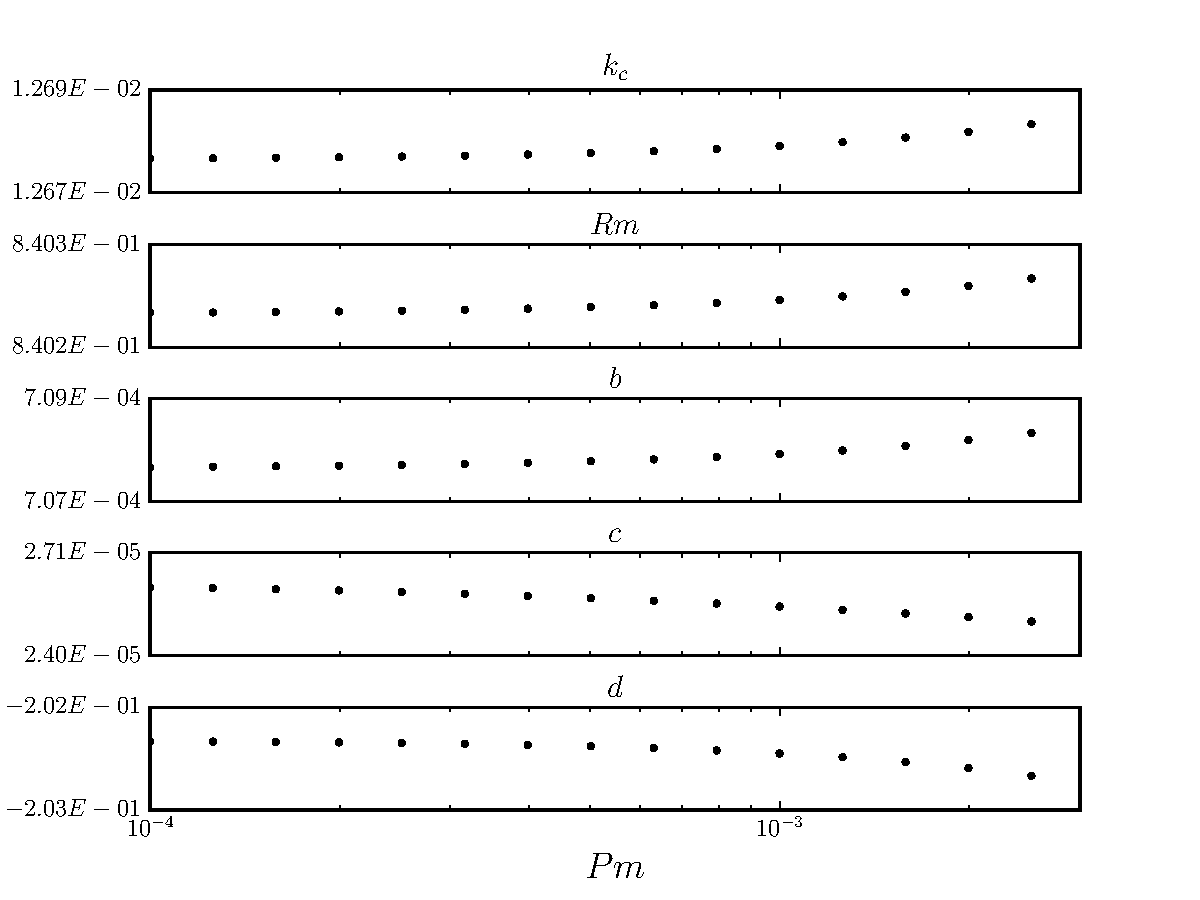
\includegraphics[width=\columnwidth]{../figures/widegap_coeffs_by_Pm.pdf}
\caption{Critical parameters $k_c$ and $\reym$, and coefficients of the Ginzburg-Landau equation (Equation \ref{eq:gle}) as a function of $Pm$. Note the very weak dependence of the coefficients on $Pm$. The saturation amplitude of the standard MRI system is very insensitive to $Pm$ in the wide gap case.}\label{fig:coefficients}
\end{figure}

\begin{figure*}
\centering
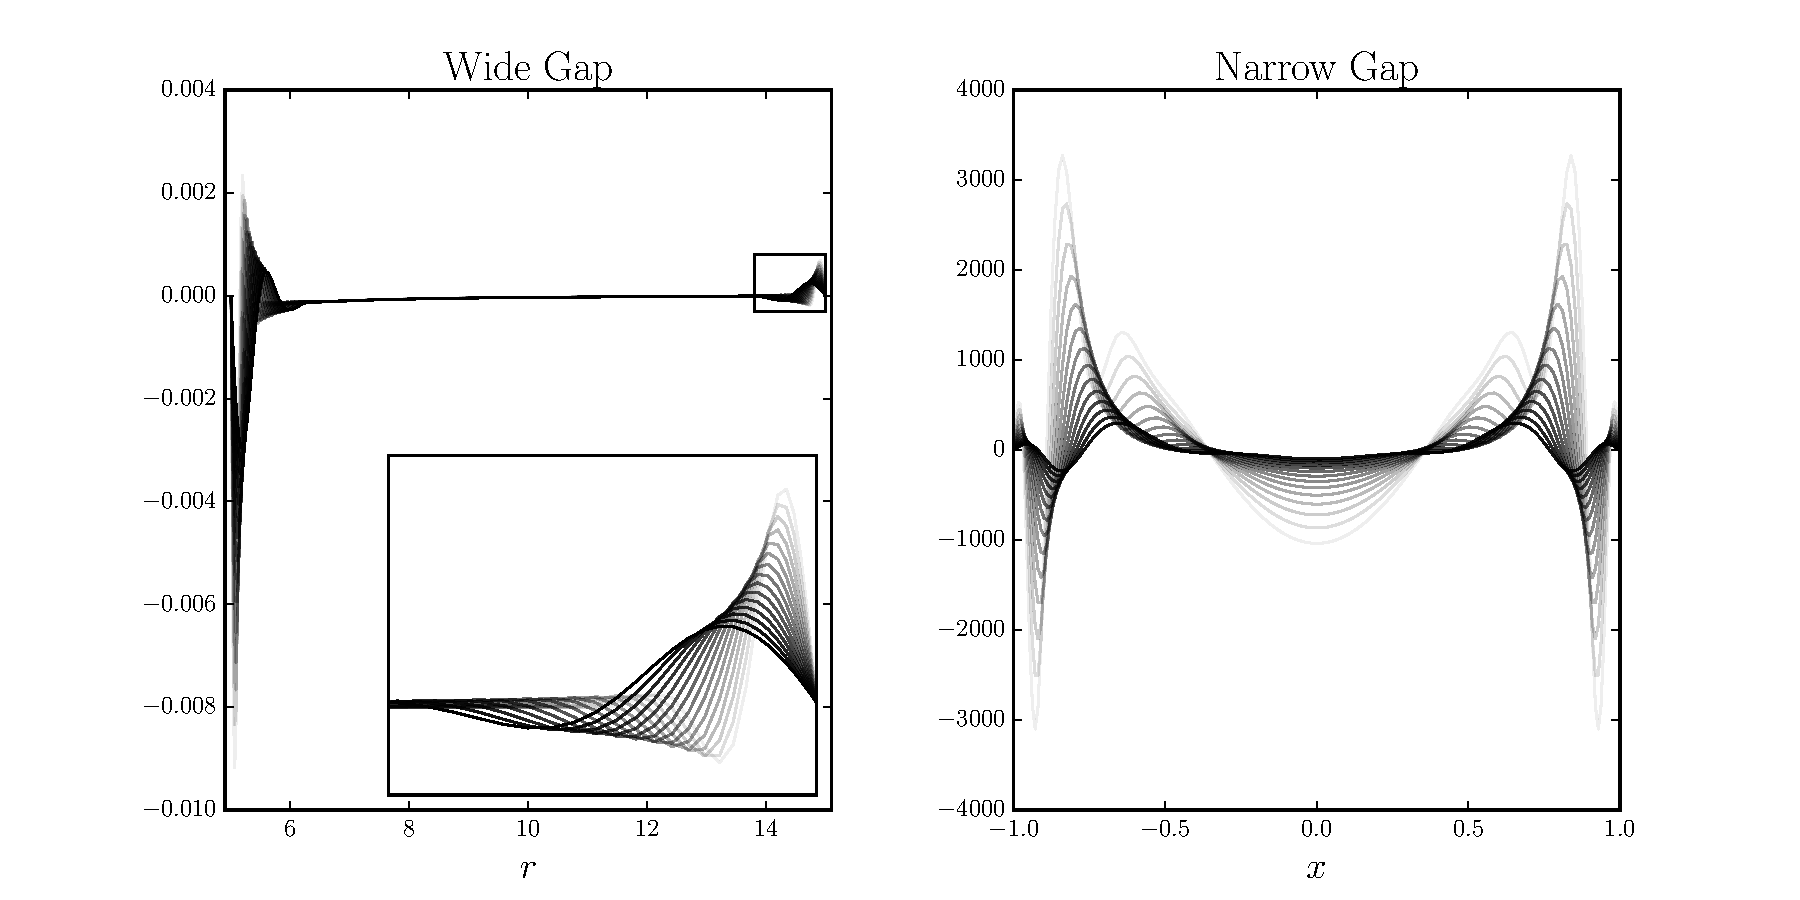
\includegraphics[width=\textwidth]{../figures/wide_narrow_gap_N31_B.pdf}
\caption{Nonlinear term $N_{31}^{(B)}$ for the wide gap (left) and narrow gap (right) standard MRI. Each line represents a run for a different $Pm$, from $Pm = 1E-4$ (darkest) to $Pm \sim 1E-3$ (lightest). Inlaid plot in wide gap case shows a zoomed-in view of the boundary layer at the outer boundary ($r_2$). In the narrow gap case the boundary layer strongly affects the bulk of the flow, while in the wide gap case the flow in the center of the channel is relatively unaffected by width of the boundary layers.}\label{fig:wide_narrow_N31B}
\end{figure*}

Just as in the weakly nonlinear analyses of \citei{Umurhan:2007hs} and \citei{Clark:2016}, we tune the system away from marginality by taking $B_0 \rightarrow B_0\left(1 - \epsilon^2\right)$, where $\epsilon \ll 1$. We parameterize scale separation as $Z = \epsilon z$ and $T = \epsilon^2 t$, where $Z$ and $T$ are slowly varying spatial and temporal scales, respectively. We group the fluid variables into a state vector $\mathbf{V} = \left[\Psi, u, A, B\right]^{\mathrm{T}}$, such that the full nonlinear system can be expressed as

\beq\label{eq:unperturbed_matrix_eqns}
\mathcal{D}\partial_t\mathbf{V} + \mathcal{L}\mathbf{V} + \epsilon^2 \widetilde{\mathcal{G}} \mathbf{V} + \xi \widetilde{\mathcal{H}} \mathbf{V} +  \mathbf{N} = 0,
\eeq

where $\mathcal{D}$, $\mathcal{L}$, and $\widetilde{\mathcal{G}}$ are matrices defined in Appendix \ref{app:basic_equations}, and $\mathbf{N}$ is a vector containing all nonlinear terms defined in Appendix \ref{app:nonlinear_terms}. We then expand the variables in a perturbation series $\mathbf{V} = \epsilon \mathbf{V}_1 + \epsilon^2 \mathbf{V}_2 + \epsilon^3 \mathbf{V}_3 + h.o.t.$ The perturbed system can then be expressed at each order by the equations

\begin{align}
\mathcal{O}(\epsilon)&: \mathcal{L} \mathbf{V}_1 + \xi \widetilde{\mathcal{H}} \mathbf{V}_1 + \mathcal{D} \partial_t \mathbf{V}_1 = 0 \label{eq:ordere}\\
\mathcal{O}(\epsilon^2)&: \mathcal{L} \mathbf{V}_2 + \xi \widetilde{\mathcal{H}} \mathbf{V}_2 + \widetilde{\mathcal{L}}_1 \partial_Z \mathbf{V}_1 + \xi \mathcal{H} \partial_Z \mathbf{V}_1 + \mathbf{N}_2 = 0 \\\label{eq:ordere2}
\mathcal{O}(\epsilon^3)&: \mathcal{L}\mathbf{V}_3 + \xi \widetilde{\mathcal{H}} \mathbf{V}_3 + \mathcal{D} \partial_T \mathbf{V}_1 + \widetilde{\mathcal{L}}_1 \partial_Z \mathbf{V}_2\nonumber \\ 
&+ \xi \mathcal{H}\partial_Z \mathbf{V}_2 + \widetilde{\mathcal{L}}_2 \partial_Z^2 \mathbf{V}_1 - \xi \widetilde{\mathcal{H}} \mathbf{V}_1 + \widetilde{\mathcal{G}} \mathbf{V}_1 + \mathbf{N}_3 = 0. \\\label{eq:ordere3}
\end{align}

See Appendix \ref{app:basic_equations} for the definition of matrices and nonlinear vectors, and a thorough derivation. We emphasize that Equations \ref{eq:ordere} - \ref{eq:ordere3} have the same form as these equations in the narrow gap case, although the matrices (which contain all radial derivatives) are significantly different in this wide gap formulation. This is because we do not have slow variation in the radial dimension. The slow variation in $Z$ and $T$ are parameterized as an amplitude function $\alpha(Z, T)$ which modulates the flow in these dimensions. This parameterization coupled with the boundary conditions lead us to an ansatz linear solution $\mathbf{V}_1 = \alpha(Z, T) \mathbb{V}_{11}(r) e^{i k_z z} + c.c.$, where the radial variation is contained in $\mathbb{V}_{11}$. 

We solve the equations at each order using Dedalus, an open source pseudospectral code (Burns et al. in prep). Because our domain is bounded only radially and not vertically, we solve the radial dimension on a basis of Chebyshev polynomials, and the vertical dimension on a Fourier series basis. We solve Equation \ref{eq:ordere} as a linear eigenvalue problem, and Equations \ref{eq:ordere2} and \ref{eq:ordere3} as linear boundary value problems. %should i mention spurious eigenvals? 
To analyze the MRI system at marginality, we fix the parameters listed in Table \ref{table:parameters} and determine the critical $\reym$ and $k_z$ by repeatedly solving Equation \ref{eq:ordere} to determine the smallest parameter values for which the fastest growing mode is zero. That is, we solve the linear eigenvalue problem for eigenvalues $\sigma = \gamma + i \omega$. Figure \ref{fig:growth_rates} shows linear MRI growth rates $\gamma$ in the $(\reym, k_z)$ plane. For the fiducial standard MRI parameters in Table \ref{table:parameters} we find critical parameters $\reym_c = 0.84$, $k_c = 0.0127$. 

%We defer full expressions and derivations thereof to the Appendix, and focus here on features of the wide gap system which distinguish it from the narrow gap limit.

The result of the weakly nonlinear analysis is a single amplitude equation for $\alpha$. This amplitude equation is found by enforcing a solvability criterion on Equation \ref{eq:ordere3}. We find

\beq
 \label{eq:gle}
\partial_T \alpha = b \alpha + d \partial_Z^2 \alpha - c \alpha \left|\alpha^2\right|,
\eeq

a Ginzburg-Landau equation (GLE). The GLE governs the weakly nonlinear amplitude behavior in a wide range of physical systems, including the narrow gap MRI (\citei{Umurhan:2007hs}), Rayleigh-B\'enard convection, and hydrodynamic Taylor Couette flow. We emphasize that this is a model equation, valid only near marginality (e.g. \citei{Cross:1993el}). The dynamics of the GLE are determined by its coefficients, which are in turn determined by the linear eigenfunctions and nonlinear vectors plotted in Figures \ref{fig:linear_eigenfunctions} and \ref{fig:N2_N3}. Equation \ref{eq:gle} contains three coefficients: $b$, which determines the linear growth rate of the system, $d$, a diffusion coefficient, and $c$, the coefficient of the nonlinear term. When all of the coefficients of Equation \ref{eq:gle} are real, this is known as the real GLE, although the amplitude $\alpha$ remains complex. The real GLE is subject to several well-studied instabilities, including the Ekhaus and Zig-Zag instabilities. When the coefficients are complex, we have the complex GLE, a source of even richer phase dynamics than its real counterpart (e.g. \citei{Aranson:2002}).

%For the standard MRI we derive a real GLE, and for the helical MRI we derive a complex GLE. 
 %This complex GLE is a natural form for the HMRI, as it is a traveling wave instability.

\section{Results and Discussion}

\begin{figure*}
\centering
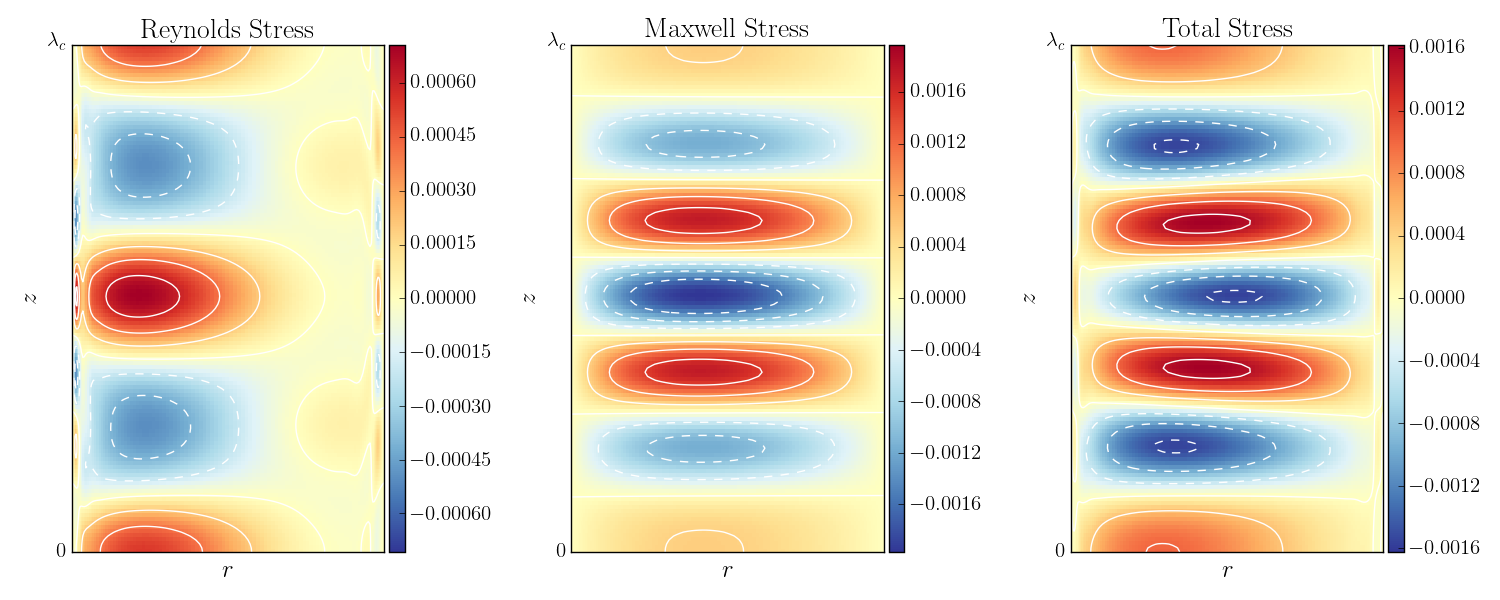
\includegraphics[width=\textwidth]{../figures/widegap_rey_max_tot_stresses.png}
\caption{Reynolds ($\mathbb{T}_{R} = u_r u_\phi$), Maxwell ($\mathbb{T}_{M} = -\frac{2}{\beta} B_r B_\phi$), and total stress ($\mathbb{T} = \mathbb{T}_{R} + \mathbb{T}_{M}$) for the fiducial standard MRI case. }
\end{figure*}

\begin{figure}
\centering
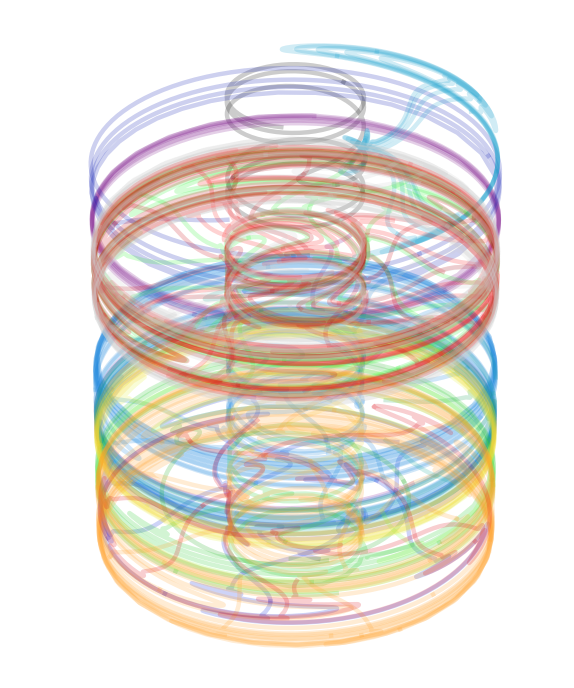
\includegraphics[width=\columnwidth]{../figures/widegap_3D_vel_screenshot.png}
\caption{Visualization of the velocity perturbation field in the fiducial SMRI case. The three dimensional path of twenty randomly placed tracer particles is plotted, where the particle velocity is defined as the total (first + second order) velocity perturbation. This is meant to be a visualization only of the velocity field, so the particle motion feels no contribution from the magnetic field.}
\end{figure}

\subsection{Standard MRI}

For the standard MRI we derive a real GLE. Here we note a departure from the behavior of the narrow gap system. The purely conducting boundary condition states that the axial component of the current ($\mathbf{J}_z = [\nabla \times \mathbf{B}]_z)$ must be zero at the walls. In the thin gap geometry, the purely conducting boundary condition on the azimuthal magnetic field is $\partial_x(B_y) = 0$ for axisymmetric perturbations. A spatially constant azimuthal field satisfies both the thin-gap MRI equations and this boundary condition. This neutral mode is formally included in the analysis of \citei{Umurhan:2007hs} and yields a second amplitude equation in the form of a simple diffusion equation. This amplitude equation decouples from the GLE because of the translational symmetry of the thin-gap geometry. Because that symmetry is not preserved in the wide-gap case, \citeauthor{Umurhan:2007hs} postulate that slow variation in the wide-gap geometry will be governed by two coupled amplitude equations. %However, the wide-gap conducting boundary condition $J_z = \frac{1}{r} \partial_r (r B_\phi) = 0$, together with the purely geometric term in Equation \ref{eq:Bphi_perturbed}, conspire to prevent the wide-gap geometry from sustaining a neutral mode. 
However, the purely geometric term in Equation \ref{eq:Bphi_perturbed} prevents the wide-gap geometry from sustaining a neutral mode. We note that a neutral mode of the form $B_\phi(r) \propto \frac{1}{r}$ would exist in a resistance-free approximation.

The preservation of symmetries in the thin-gap geometry is worth a closer look, as its absence in the wide gap case is the source of many differences in the systems. \citei{Latter:2015} point out that in the ideal limit ($\nu, \eta \rightarrow 0$), the linearized system described by the lefthand side of Equations \ref{eq:Psi_perturbed} - \ref{eq:Bphi_perturbed} can be expressed as a Shr{\"o}dinger equation for the radial velocity. Similarly combining equations to obtain a single expression for $\Psi$, we find that the thin-gap limit linear ideal MRI can be expressed as

\beq
\partial_x^2 \Psi + k_z^2 \mathrm{U}(x) \Psi = 0
\eeq 

where $\mathrm{U}(x) = {3}/{v_A^2 k_z^2} + 1$ at marginality. When no-slip radial boundary conditions are applied, the thin-gap MRI system resembles a particle in a box with a radially constant potential well. Thus thin-gap linear MRI modes must be eigenstates of parity. These symmetries are preserved in the nonlinear MRI terms because they are nonlinear combinations of lower-order eigenfunctions. In the wide gap case, the ``potential" $\mathrm{U}(r)$ varies with $r$, so symmetric and antisymmetric modes are no longer required.

The nonlinear terms, detailed in Appendix \ref{app:nonlinear_terms}, represent an interesting departure from the thin-gap theory. The thin-gap nonlinear terms at both second and third orders are linear combinations of Jacobians. The nonlinear terms in the wide-gap case differ from their thin-gap analogues with in the addition of vertical advective terms. These terms derive from the advective derivatives in the momentum and induction equations, but are filtered out in the thin-gap approximation. These advective terms allow the nonlinear contributions at both second and third order (i.e. N$_2$ and N$_3$) not to individually satisfy the boundary conditions on $\Psi$ and $u$. %(I'm just guessing but this may lead to higher torque on inner cylinder -- should calculate) 

We examine the behavior of the wide gap MRI system as a function of $Pm$. Figure \ref{fig:coefficients} shows the critical parameters $k_c$ and $\reym$ as a function of $Pm$, as well as the coefficients $b$, $c$, and $d$. The GLE coefficients are remarkably insensitive to $Pm$. From Equation \ref{eq:gle} it is readily apparent that the asymptotic saturation amplitude is $\alpha_{s} = \pm \sqrt{b/c}$, so we conclude that the saturation amplitude of the MRI is only very weakly dependent on $Pm$. Note that because $\reym$ is essentially constant as a function of $Pm$, the saturation amplitude is equivalently insensitive to $\reye^{-1}$. This is in stark contrast to the narrow gap behavior of the system. For these same boundary conditions, \citeauthor{Umurhan:2007hs} (\citeyear{Umurhan:2007hs}) find that the narrow gap saturation amplitude scales as $Pm^{-4/3}$. They find that this amplitude dependence is driven by the $Pm^{1/3}$ dependence of the linear boundary layer. Boundary layer analysis similarly reveals a $\nu^{1/3}$ dependence for the radial extent of the boundary layer (\citei{Goodman:2002ix}). Why does the $Pm$ scaling of the boundary layer width not translate to a stronger $Pm$ scaling for the saturation amplitude in the wide gap case? The boundary layer in the wide gap case is strongly localized at the walls, i.e. $r_1$ and $r_2$. Figure \ref{fig:wide_narrow_N31B} shows the structure of the third-order nonlinear term $N_{31}^{(B)}$ as a function of $Pm$ for both the narrow and wide gap standard MRI. $N_{31}$ is the vector that determines the GLE coefficient $c$ (see Appendix \ref{app:basic_equations} for the wide gap case, and \citei{Umurhan:2007hs}, \citei{Clark:2016} for the narrow gap equations). Clearly, the boundary layers scale with $Pm$ in both the wide and narrow gap MRI. However, in the narrow gap case this scaling extends prominently into the center of the channel, whereas for the wide gap case the bulk of the flow is relatively unaffected by the boundary layer scaling. 

%\section{Channel Modes}
%Channel modes are radially independent linear MRI modes which are, under certain conditions, exact nonlinear solutions to the MRI equations. 

\subsection{Helical MRI}

When $\xi$ in Equation \ref{eq:unperturbed_matrix_eqns} is not equal to zero, the helical MRI arises. We examine a single fiducial helical MRI case, for the parameters listed in Table \ref{table:parameters}. At the conclusion of the weakly nonlinear analysis, we find that the coefficients of Equation \ref{eq:gle} are $b = $, $d = $, and $c = $, i.e. complex. The marginal helical MRI is thus described by a complex GLE. This difference in character between the amplitude equations that modulate the weakly nonlinear standard and helical MRI is a consequence of the same property that makes the helical MRI an overstability. 


\clearpage
\appendix

\section{A. Detailed Equations}\label{app:basic_equations}

Here we detail the perturbation analysis described in Section \ref{sec:wnl_analysis}. The linear system is described by Equation \ref{eq:unperturbed_matrix_eqns}, where 

\beq
\mathcal{L} = \mathcal{L}_0 + \mathcal{L}_1 \partial_z + \mathcal{L}_2 \partial_z^2 + \mathcal{L}_3 \partial_z^3 + \mathcal{L}_4 \partial_z^4,
\eeq

\beq
\widetilde{\mathcal{G}} = - \mathcal{G} \partial_z - \mathcal{L}_3 \partial_z^3,
\eeq

\beq
\widetilde{\mathcal{H}} = \mathcal{H} \partial_z,
\eeq

and the constituent matrices are defined as 

\beq
\mathcal{L}_0 = \left[\begin{matrix}
-\frac{1}{\reye} (-\frac{3}{r^4} \partial_r + \frac{3}{r^3}\partial_r^2 - \frac{2}{r^2}\partial_r^3 + \frac{1}{r}\partial_r^4) & 0 & 0 & 0 \\
0 & -\frac{1}{\reye} (\partial_r^2 + \frac{1}{r}\partial_r - \frac{1}{r^2}) & 0 & 0 \\
0 & 0 & -\frac{1}{\reym} (\partial_r^2 - \frac{1}{r} \partial_r) & 0 \\
0 & 0 & 0 & -\frac{1}{\reym} (\partial_r^2 + \frac{1}{r}\partial_r - \frac{1}{r^2}) \\
\end{matrix}\right]
\eeq

\beq
\mathcal{L}_1 = \left[\begin{matrix}
0 & -\frac{2}{r} u_0 & \frac{2}{\beta} (\frac{1}{r^2} \partial_r - \frac{1}{r}\partial_r^2) & 0 \\
\frac{1}{r^2} u_0 + \frac{1}{r}\partial_r u_0 & 0 & 0 & -\frac{2}{\beta} \\
-1 & 0 & 0 & 0 \\
0 & -1 & \frac{1}{r^2} u_0 - \frac{1}{r} \partial_r u_0 & 0 \\
\end{matrix}\right]
\eeq


\beq
\mathcal{L}_2 = \left[\begin{matrix}
-\frac{1}{\reye} (-\frac{2}{r^2}\partial_r + \frac{2}{r}\partial_r^2) & 0 & 0 & 0 \\
0 & -\frac{1}{\reye} & 0 & 0 \\
0 & 0 & -\frac{1}{\reym} & 0 \\
0 & 0 & 0 & -\frac{1}{\reym} \\
\end{matrix}\right]
\eeq

\beq
\mathcal{L}_3 = \left[\begin{matrix}
0 & 0 & -\frac{2}{\beta}\frac{1}{r} & 0 \\
0 & 0 & 0 & 0 \\
0 & 0 & 0 & 0 \\
0 & 0 & 0 & 0 \\
\end{matrix}\right]
\eeq

\beq
\mathcal{L}_4 = \left[\begin{matrix}
-\frac{1}{\reye}\frac{1}{r} & 0 & 0 & 0 \\
0 & 0 & 0 & 0 \\
0 & 0 & 0 & 0 \\
0 & 0 & 0 & 0 \\
\end{matrix}\right]
\eeq

\beq
\mathcal{G} = \left[\begin{matrix}
0 & 0 & \frac{2}{\beta}(\frac{1}{r^2}\partial_r - \frac{1}{r}\partial_r^2) & 0 \\
0 & 0 & 0 & -\frac{2}{\beta} \\
-1 & 0 & 0 & 0 \\
0 & -1 & 0 & 0 \\
\end{matrix}\right]
\eeq

\beq
\mathcal{H} = \left[\begin{matrix}
0 & 0 & 0 & \frac{2}{\beta} \frac{2}{r^2} \\
0 & 0 & 0 & 0 \\
0 & 0 & 0 & 0 \\
-\frac{2}{r^3} & 0 & 0 & 0 \\
\end{matrix}\right]
\eeq

\beq
\mathcal{D} = \left[\begin{matrix}
\frac{1}{r}\partial_r^2 + \frac{1}{r}\partial_z^2 - \frac{1}{r^2}\partial_r & 0 & 0 & 0 \\
0 & 1 & 0 & 0 \\
0 & 0 & 1 & 0 \\
0 & 0 & 0 & 1 \\
\end{matrix}\right]
\eeq

\section{B. Nonlinear Terms}\label{app:nonlinear_terms}

Here we detail the perturbative expansion of the nonlinear vector $\mathbf{N}$ in Equation \ref{eq:unperturbed_matrix_eqns}. 

\beq
\mathbf{N} = \epsilon^2 \mathbf{N}_2 + \epsilon^3 \mathbf{N}_3
\eeq

\beq
N_2^{\Psi}  = J(\Psi_1, \frac{1}{r^2} \nabla^2 \Psi_1) + J(\Psi_1, -\frac{2}{r^3}\partial_r\Psi_1)
- \frac{2}{\beta} J (A_1, \frac{1}{r^2} \nabla^2 A_1) - \frac{2}{\beta} J(A_1, -\frac{2}{r^3} \partial_r A_1) - \frac{2}{r} u_1 \partial_z u_1 + \frac{2}{\beta} \frac{2}{r} B_1 \partial_z B_1
\eeq

\beq
\begin{split}
N_2^{u} = \frac{1}{r} J\left(\Psi_1, u_1\right) - \frac{1}{r} \frac{2}{\beta} J\left(A_1, B_1\right) + \frac{1}{r^2} u_1 \partial_z \Psi_1 - \frac{2}{\beta}\frac{1}{r^2} B_1 \partial_z A_1
\end{split}
\eeq

\beq
N_2^A = -\frac{1}{r} J\left(A_1, \Psi_1\right)
\eeq

\beq
N_2^B = -\frac{1}{r} J\left(A_1, u_1\right) - \frac{1}{r} J\left(B_1, \Psi_1\right) - \frac{1}{r^2} B_1 \partial_z \Psi_1 + \frac{1}{r^2} u_1 \partial_z A_1
\eeq

\beq
\begin{split}
N_3^{\Psi} & = J(\Psi_1, \frac{1}{r^2} \nabla^2 \Psi_2) + J(\Psi_2, \frac{1}{r^2} \nabla^2\Psi_1) + 2 J (\Psi_1, \frac{1}{r^2}\partial_Z\partial_z \Psi_1) + J(\Psi_1, -\frac{2}{r^3}\partial_r \Psi_2) + J(\Psi_2, -\frac{2}{r^3}\partial_r \Psi_1) \\
& + \widetilde{J}(\Psi_1, \frac{1}{r^2} \nabla^2 \Psi_1) + \widetilde{J} (\Psi_1, -\frac{2}{r^3}\partial_r \Psi_1) - \frac{2}{\beta} J(A_1, \frac{1}{r^2}\nabla^2 A_2) - \frac{2}{\beta} J(A_2, \frac{1}{r^2}\nabla^2 A_1) - \frac{4}{\beta} J(A_1, \frac{1}{r^2}\partial_Z\partial_z A_1) \\ & - \frac{2}{\beta} J(A_1, -\frac{2}{r^3} \partial_r A_2 ) 
 - \frac{2}{\beta} J(A_2, -\frac{2}{r^3} \partial_r A_1) - \frac{2}{\beta} \widetilde{J} (A_1, \frac{1}{r^2} \nabla^2 A_1) - \frac{2}{\beta} \widetilde{J} (A_1, -\frac{2}{r^3} \partial_r A_1) \\
& - \frac{2}{r} u_1 \partial_z u_2 - \frac{2}{r} u_2 \partial_z u_1 - \frac{2}{r} u_1 \partial_Z u_1 + \frac{2}{\beta}\frac{2}{r} B_1\partial_z B_2 + \frac{2}{\beta}\frac{2}{r} B_2 \partial_z B_1 + \frac{2}{\beta} \frac{2}{r} B_1 \partial_Z B_1
\end{split}
\eeq

\beq
\begin{split}
N_3^u & = \frac{1}{r}J\left(\Psi_1, u_2\right) + \frac{1}{r}J\left(\Psi_2, u_1\right) + \frac{1}{r}\widetilde{J} \left(\Psi_1, u_1\right) - \frac{1}{r}\frac{2}{\beta} J\left(A_1, B_2\right) - \frac{1}{r} \frac{2}{\beta} J\left(A_2, B_1\right) - \frac{1}{r}\frac{2}{\beta}\widetilde{J}\left(A_1, B_1\right) \\
& + \frac{1}{r^2} u_1\partial_z \Psi_2 + \frac{1}{r^2} u_2 \partial_z \Psi_1 + \frac{1}{r^2} u_1 \partial_Z \Psi_1 - \frac{2}{\beta} \frac{1}{r^2} B_1 \partial_z A_2 - \frac{2}{\beta} \frac{1}{r^2} B_2 \partial_z A_1 - \frac{2}{\beta} \frac{1}{r^2} B_1 \partial_Z A_1
\end{split}
\eeq

\beq
N_3^A = -\frac{1}{r} J\left(A_1, \Psi_2\right) - \frac{1}{r}J\left(A_2, \Psi_1\right) - \frac{1}{r} \widetilde{J}\left(A_1, \Psi_1\right)
\eeq

\beq
\begin{split}
N_3^B & = - \frac{1}{r} J\left(A_1, u_2\right) - \frac{1}{r} J\left(A_2, u_1\right) - \frac{1}{r}\widetilde{J}\left(A_1, u_1\right) - \frac{1}{r} J\left(B_1, \Psi_2\right) - \frac{1}{r} J\left(B_2, \Psi_1\right) - \frac{1}{r} \widetilde{J} \left(B_1, u_1\right) \\ & - \frac{1}{r^2} B_1\partial_z \Psi_2 - \frac{1}{r^2} B_2 \partial_z \Psi_1 - \frac{1}{r^2} B_1 \partial_Z \Psi_1 + \frac{1}{r^2} u_1 \partial_z A_2 + \frac{1}{r^2} u_2 \partial_z A_1 + \frac{1}{r^2} u_1 \partial_Z A_1
\end{split}
\eeq


\bibliographystyle{plain}

\begin{thebibliography}{53}
\expandafter\ifx\csname natexlab\endcsname\relax\def\natexlab#1{#1}\fi

\bibitem[{Aranson \& Kramer(2002)}]{Aranson:2002}
Aranson, I.S. \& Kramer, L., 2002, Rev. Mod. Phys. 74, 99

\bibitem[{Armitage(2010)}]{Armitage:2010}
Armitage, P. 2010, ARA\&A, 49, 195

\bibitem[{Bai(2011)}]{Bai:2011cm}
Bai, X. 2011, ApJ 739, 50

\bibitem[{Balbus \& Hawley(1991)}]{Balbus:1991vs}
Balbus, S A and Hawley, J F, 1991, The Astrophysical Journal, 376, 214

\bibitem[{Chandrasekhar(1960)}]{Chandrasekhar:1960wh}
Chandrasekhar, S. 1960, Proceedings of the National Academy of Sciences of the United States of America, 46, 253

\bibitem[{Clark \& Oishi(2016a)}]{Clark:2016}
Clark, S.E. and Oishi, J.S., 2016, in prep

\bibitem[{Cross \& Hohenberg(1993)}]{Cross:1993el}
Cross, M. C., \& Hohenberg, P. C., 1993, Rev. Mod. Phys. 65, 851

\bibitem[{Ebrahimi et al.(2009)}]{Ebrahimi:2009ey}
Ebrahimi, F., Prager, S.C., Schnack, D.D

\bibitem[{Fleming \& Stone(2003)}]{Fleming:2003fs}
Fleming, T. \& Stone, J. 2003, ApJ 585, 908

\bibitem[{Flock et al.(2013)}]{Flock:2013}
Flock, M., Fromang, S., Gonz\'alez, M., Commer\c{c}on, B. A\&A 560, A43

\bibitem[{Gissinger et al.(2011)}]{Gissinger:2011td}
Gissinger, C, Ji, H, Goodman, J, 2011, Phys. Rev. E 84, 026308

\bibitem[{Gissinger et al.(2012)}]{Gissinger:2012gc}
Gissinger, C, Goodman, J, \& Ji, H, 2012, Physics of Fluids 24, 074109

\bibitem[{Goodman \& Ji(2002)}]{Goodman:2002ix}
Goodman, J. \& Ji, H., 2002, JFM, 462, 365

\bibitem[Goodman \& Xu(1994)]{Goodman:1994ul}
Goodman, J, Xu, G, 1994, ApJ, 432, 213

\bibitem[{Hollerbach(2009)}]{Hollerbach:2009ig}
Hollerbach, R, Proc. R. Soc. A, 2009, 465, 2107

\bibitem[{Hollerbach \& R\"udiger(2005)}]{Hollerbach:2005tr}
Hollerbach, R. \& R\"udiger, G., 2005, Phys. Rev. Lett. 95, 124501

\bibitem[{Ji et al.(2001)}]{Ji:2001kd}
Ji, H, Goodman, J, Kageyama, A, Mon. Not. R. Astron. Soc., 2001, 325, 1

\bibitem[{Kirillov \& Stefani(2013)}]{Kirillov:2013}
Kirillov, O, \& Stefani, F, 2013, Phys. Rev. Lett. 111, 061103

\bibitem[{Knobloch \& Julien(2005)}]{Knobloch:2005ba}
Knobloch, E, Julien K, 2005, Physics of Fluids, 17, 094106

\bibitem[{Latter et al.(2015)}]{Latter:2015}
Latter, H.N., Fromang, S., \& Faure, J., 2015, MNRAS 453, 3257

\bibitem[{Lesur et al.(2013)}]{Lesur:2013}
Lesur, G., Ferreira, J., \& Ogilvie, G. I. 2013, A\&A 550, A61

\bibitem[{Liu et al.(2006)}]{Liu:2006}
Liu, W, Goodman, J, Herron, I, and Ji, H, 2006, Phys. Rev. E 74, 056302

\bibitem[Pessah(2010)]{Pessah:2010ic}
Pessah, M, 2010, ApJ, 716, 1012

\bibitem[{R\"udiger \& Hollerbach(2007)}]{Rudiger:2007}
R\"udiger, G, \& Hollerbach, R, Phys. Rev. E 76, 068301

\bibitem[{Schartman et al.(2009)}]{Schartman:2009df}
Schartman, E, Ji, H, Burin, M J, Rev Sci Instrum, 2009, 80, 024501

\bibitem[{Shakura \& Sunyaev(1973)}]{Shakura:1973wg}
Shakura, N I and Sunyaev, R A, Astronomy \& Astrophysics, 1973, 24, 337

\bibitem[{Sisan et al.(2004)}]{Sisan:2004ig}
Sisan, D R, Mujica, N, Tillotson, W A, Huang Y-M, Dorland, W, Hassam, A B, Antonsen, T M, Lathrop, D P, Phys Rev Lett, 2004, 93, 11

\bibitem[{Stefani et al.(2006)}]{Stefani:2006iv}
Stefani, F, Gundrum, T, Gerbeth, G, R\"udiger, G, Schultz, M, Szklarski, J, Hollerbach, R, Phys Rev Lett, 2006, 97, 184502

\bibitem[{Stefani et al.(2009)}]{Stefani:2009hp}
Stefani, F, Gerbeth, G, Gundrum, T, Hollerbach, R, Priede, J, R\"udiger, G, and Szklarski, J, Phys Rev E, 80, 066303

\bibitem[{Suzuki \& Inutsuka(2014)}]{Suzuki:2014vh}
Suzuki, T.K. \& Inutsuka, S. 2014, ApJ 784, 121

\bibitem[{Umurhan et al.(2007a)}]{Umurhan:2007dz}
Umurhan, O.M., Regev, O., Menou, K., 2007, Phys. Rev. Letters, 98, 034501

\bibitem[{Umurhan et al.(2007b)}]{Umurhan:2007hs}
Umurhan, O.M., Regev, O., Menou, K., 2007, Phys. Rev. E, 76, 036310


\end{thebibliography}

\end{document}

